%!TEX root = main.tex
\chapter{Multidimensional Root-finding and Optimization}
\begin{center}
Guangting Yu, University of Michigan - Shanghai Jiao Tong University Joint Institute, Minhang, Shanghai, 200135, China
\end{center}


\section*{Abstract}
This paper explores numerical methods in higher dimemsions, including the fixed-point iteration, Newton's method and secant method.
A robust schema which involves the combination of these methods is introduced to find roots of higher dimensional functions.
Applications to system of equations in \(\R^2\) and \(\R^3\) are studied to illustrate these methods.
An application to non-linear regression is optimized by using the schema.
The performances such as convergence and sensitivity with respect to the initial guess of these methods are also studied and compared.



\section{Introduction}
Finding roots of functions in higher dimensions is similar to the methods in one dimension.
In this paper, our goal is to solve the following problems, including two systems of equations and a non-linear optimization from the non-linear regression model.


\subsection{System of Equations}
The first system is in \(\R^2\).
\begin{equation}\label{eqn1}
\begin{aligned}
x_1^2-x_2&=0\\
x_1^2+x_2^2&=1
\end{aligned}
\end{equation}
The second system is in \(\R^3\)
\begin{equation}\label{eqn2}
\begin{aligned}
3x_1-\cos(x_2x_3)&=\frac{1}{2}\\
x_1^2-625x_2^2&=\frac{1}{4}\\
\exp(-x_1x_2)+20x_3&=1-\frac{10}{3}\pi
\end{aligned}
\end{equation}



\subsection{Non-linear Regression}
The following function denote some physical relationship between the variables \(y\) and \(x\).
\[ y=\alpha\exp\left(\frac{\beta}{x+\gamma}\right), \]
where \(\alpha,\beta,\gamma\) are unknown parameters in \(\R\).
Suppose the following data are obtained from an experiment, and we want to find the best estimate for \(\alpha,\beta,\gamma\) by minimizing the sum of square errors
\begin{equation}\label{sse}
E=\sum_{i=1}^{n} \left[  y_i-\alpha\exp\left(\frac{\beta}{x_i+\gamma}\right) \right]^2.
\end{equation}
The data is given in
\ifnum\webview=1
	\begin{table}[H]
\else
	\begin{table}[htbp]
\fi
	\centering
	\begin{tabular}{ccccccccc}
	\hline
	\(x\)	&	50	&	55	&	60	&	65	&	70	&	75	&	80	&	85	\\
	\(y\)	&	34780	&	28610	&	23650	&	19630	&	16370	&	13720	&	11540	&	9744			\\	\hline\hline
	\(x\)	&	90	&	95	&	100	&	105	&	110	&	115	&	120	&	125 \\
	\(y\)	&	8261	&	7030	&	6005	&	5147	&	4427	&	3820	&	3307	&	2872	\\	\hline
	\end{tabular}
	\caption{Data for non-linear regression}
	\label{regression}
	\end{table}





\section{Analysis}
\subsection{Reduction of Dimensions}
The reduction of dimensions is implemented by the idea to apply substitutions to reduce the number of equations and unknowns.
The best scenerio is that the system of equations can be reduced to only one equation with only one unknown. 
Then the problem can be solved by the methods in one dimension.

Specifically, the two systems (\ref{eqn1}) and (\ref{eqn2}) can both be reduced to one dimension.
In (\ref{eqn1}), we apply the substitution
\[ x_2=x_1^2, \]
and the system is reduced to
\begin{equation}\label{eqn1reduce}
x_1^4+x_1^2-1=0,
\end{equation}
which can be solved algebraically.
The real roots are
\[ x_1=\pm\sqrt{\frac{\sqrt{5}-1}{2}}, \quad x_2=\frac{\sqrt{5}-1}{2}. \]
Two other roots exist, but \(x_1\) is a complex number, so we don't list them here, since the numerical methods we discuss cannot find them.
In (\ref{eqn2}), we apply the trignometric substitution
\[ \begin{aligned} x_1&=\frac{1}{2}\sec t \\ x_2&=\frac{1}{50}\tan t\\
x_3&=\frac{1}{20}-\frac{\pi}{6}-\frac{1}{20}\exp\left(-\frac{\sec t\tan t}{100} \right) \end{aligned}. \]
Then the system of equations is reduced to
\begin{equation}\label{eqn2reduce}
3\sec t-2\cos\left\{ \frac{\tan t}{1000} \left[ 1-\frac{10}{3}\pi-\exp\left(-\frac{\sec t\tan t}{100} \right) \right] \right\}-1=0. 
\end{equation}
Furthermore, this is periodic with period \(2\pi\), so we just need to find roots in the interval \([-\pi,\pi]\).

\subsection{Generalization of Methods in Single Dimension}
In general, the reduction of dimensions does not work, since there are equations that cannot be transformed to express a variable in explicit form.
Thus, the numerical methods are still needed to solve the higher dimensional system of equations.
Here, we just generalize three methods to higher dimensions: fixed-point iteration,	Newton's method, and secant method.



\subsubsection{Fixed-point iteration}
Suppose we have the function
\[ F(x)=G(x)-x, \quad G:\mathcal{D}\subseteq\R^{n}\to\R^n, \]
where \(F(x)=0\) is the system of functions to solve.
The the fixed-point iteration
\[ x_0\in\mathcal{D}, \quad x_{k}=G(x_{k-1}), \quad k=1,2,3,\cdots  \]
converges to the root \(x^*\) where \(F(x^*)=0\) if \(G\) has the Lipschitz constant \(0\leq c<1\).
Here the Lipschitz constant is defined to be a constant that satisfies
\[ ||J_G(x_1)-J_G(x_2)|| \leq c ||x_1-x_2|| \quad \forall x_1,x_2\in\mathcal{D}, \]
where \(J_G\) denotes the Jacobian of \(G\).



\subsubsection{Newton's method}
Suppose we have the system of functions \(F(x)=0\) to solve, where \(F:\mathcal{D}\subseteq\R^{n}\to\R^n\).
Then if the series of vectors with \(x_0\in\mathcal{D}\),
\[ x_{k+1}=x_k-[J_F(x_k)]^{-1}F(x_k), \quad k=1,2,3,\cdots \]
coverges, then it coverges to a root \(x^*\) such that \(F(x^*)=0\).
Again, \(J_F\) denotes the Jacobian of \(F\).



\subsubsection{Secant method}
The secant method in higher dimension is more complicated than the one dimension case.
Suppose we have the system of functions \(F(x)=0\) to solve, where \(F:\mathcal{D}\subseteq\R^{n}\to\R^n\).
The secant method is the following iteration, with the initial guesses \(x_0\) and \(x_1\) and the initial matrix \(A_1\) defined to be
\[ A_1\coloneqq J_F(x_0)+\frac{\left[F(x_1)-F(x_0)-J_F(x_0)(x_1-x_0)\right](x_1-x_0)^T}{||x_1-x_0||_2^2} \]
And the iteration for \(k=1,2,3,\cdots\) is
\begin{align*}
	s_k&=x_{k}-x_{k-1}\\
	y_k&=F(x_k)-F(x_{k-1})\\
	A_k&=A_{k-1}+\frac{y_k-A_{k-1}s_k}{||s_k||_2^2}s_k^T\\
	w_k&=A_k^{-1}F(x_k)\\
	x_{k+1}&=x_k-w_k.
\end{align*}




\subsection{Transforming Optimization to System of Equations}
If the function \(f:\R^n\to\R\) is sufficiently smooth and convex in the absence of any constraint, we could turn the optimization problem into a root-finding problem by finding \(x^*\) such that
\[ \nabla f(x^*)=0. \]
In the non-linear regression, minimizing the sum of square errors \(E\) is equivalent to finding the root of the system of equaitons
\begin{equation}\label{eqn3}
\begin{aligned}
\partial_{\alpha}E&=0\\
\partial_{\beta}E&=0\\
\partial_{\gamma}E&=0
\end{aligned}
\end{equation}


\subsection{Combination and Construction of Robust Method}
In one dimension case, Newton's methods has the problem that the initial guess \(x_0\) is critical to the convergence of the method.
By contrast, the fixed-point iteration is sure to converge on the domain where the Lipschitz constant \(c<1\), but there is no garantee that the given system has such a property.
So transformation such as dividing by a constant can create a new function with smaller Lipschitz constant without changing the root, but determining this constant is also equivalent to finding the superme of the Jacobian matrix, which is an optimization question and the dimension does not get reduced.

Thus, in order to find a root of system of equations, the attempt by all three methods should be tried.




\section{Results}

\subsection{Solving System of Equations}
The solution to (\ref{eqn2reduce}) is easy to obtain.
Start with inital guess \(t=0\) and the solution happens to be found.
Thus the solution to (\ref{eqn2}) is
\[ x^*=\begin{pmatrix} \frac{1}{2} \\ 0 \\ -\frac{\pi}{6} \end{pmatrix}. \]
And the solution is also unique.




\subsubsection{Fixed-point Iteration}
Apply fixed-point iteration to (\ref{eqn1reduce}) near a root,
\[ G\begin{pmatrix} x_1\\ x_2\end{pmatrix}=\begin{pmatrix} x_1^2+x_1-x_2 \\ x_1^2+x_2^2+x_2-1 \end{pmatrix}, \]
we have the log in Table \ref{logeqn1fp}.
\ifnum\webview=1
	\begin{table}[H]
\else
	\begin{table}[htbp]
\fi
	\centering
	\begin{tabular}{|c|c|c|}
	\hline
	\(n\)	&	\(\hat{x}_1\)	&	\(\hat{x}_2\)	\\	\hline
	1	&	0.786000000000000		&	0.618000000000000		\\	\hline
	2	&	0.785796000000000		&	0.617720000000000		\\	\hline
	3	&	0.785551353616000		&	0.616773352016000		\\	\hline
	4	&	0.785868930767931		&	0.614273648940982		\\	\hline
	5	&	0.789185258173280		&	0.609195741070583		\\	\hline
	6	&	0.802802888820723		&	0.603128563727145		\\	\hline
	7	&	0.844166803392477		&	0.611385106409613		\\	\hline
	8	&	0.945399288932737		&	0.697794446698978		\\	\hline
	9	&	1.14138465774828		&	1.07849135205744		\\	\hline
	10	&	1.36565224263401		&	2.54439388546328		\\	\hline
	11	&	0.686264404982040		&	9.88334017765749		\\	\hline
	12	&	-8.72611693913009		&	107.034712078502		\\	\hline
	13	&	-39.6157121822585		&	11638.6094186416		\\	\hline
	14	&	-10108.8204791163		&	135470436.213763		\\	\hline
	15	&	-33292293.5552410		&	1.83522393256060e+16	\\	\hline
	16	&	-1.72438625487299e+16	&	3.36804688264319e+32	\\	\hline
	17	&	-3.94538926648279e+31	&	1.13437398036825e+65	\\	\hline
	18	&	-1.11880788390417e+65	&	1.28680432733650e+130	\\	\hline
	19	&	-3.50732462503746e+128	&	1.65586537685195e+260	\\	\hline
	20	&	-1.65463524424941e+260	&	Inf						\\	\hline
	\end{tabular}
	\caption{Log of fixed-point iteration on (\ref{eqn1reduce})}
	\label{logeqn1fp}
	\end{table}

Obviously, it does not converge.
This is a direct result from the norm of the Jacobian matrix \(||J_G||_2=3.05847254037959>1\), which means the Lipschitz constant is too large for the fixed-point iteration to converge.



\subsubsection{Newton's method}
Apply Newton's method to (\ref{eqn1reduce}) near a root,
\[ F\begin{pmatrix} x_1\\ x_2\end{pmatrix}=\begin{pmatrix} x_1^2-x_2 \\ x_1^2+x_2^2-1 \end{pmatrix}, \]
with its Jacobian matrix
\[ J_F\begin{pmatrix} x_1\\ x_2\end{pmatrix}=\begin{pmatrix} 2x_1 & -1 \\ 2x_1 & 2x_2 \end{pmatrix}\]
we have the log in Table \ref{logeqn1nt+} and \ref{logeqn1nt-}, which correspond to the root with positive \(x_1\) and the root with negative \(x_1\).
Since we have already obtained the accurate solution, we can compare the numerical results with and and find the error.
\ifnum\webview=1
	\begin{table}[H]
\else
	\begin{table}[htbp]
\fi
	\centering
	\begin{subtable}[t]{\textwidth}
		\centering
		\begin{tabular}{|c|c|c|c|c|}
		\hline
		\(n\)	&	\(\hat{x}_1\)	&	\(\hat{x}_2\)	&	Error in \(\hat{x}_1\)	&	Error in \(\hat{x}_2\)		\\	\hline
		1	&	\footnotesize	10					&	\footnotesize	1					&	\footnotesize	9.21384862224258		&	\footnotesize	0.381966011250105		\\	\hline
		2	&	\footnotesize	5.03333333333333	&	\footnotesize	0.666666666666667	&	\footnotesize	4.24718195557591		&	\footnotesize	0.0486326779167718		\\	\hline
		3	&	\footnotesize	2.57816146326080	&	\footnotesize	0.619047619047619	&	\footnotesize	1.79201008550338		&	\footnotesize	0.00101363029772439		\\	\hline
		4	&	\footnotesize	1.40894026266226	&	\footnotesize	0.618034447821682	&	\footnotesize	0.622788884904833		&	\footnotesize	4.59071787028975e-07	\\	\hline
		5	&	\footnotesize	0.923795962641458	&	\footnotesize	0.618033988749989	&	\footnotesize	0.137644584884035		&	\footnotesize	9.41469124882133e-14	\\	\hline
		6	&	\footnotesize	0.796405823822399	&	\footnotesize	0.618033988749895	&	\footnotesize	0.0102544460649757		&	\footnotesize	1.11022302462516e-16	\\	\hline
		7	&	\footnotesize	0.786217395396267	&	\footnotesize	0.618033988749895	&	\footnotesize	6.60176388432854e-05	&	\footnotesize	0						\\	\hline
		8	&	\footnotesize	0.786151380529131	&	\footnotesize	0.618033988749895	&	\footnotesize	2.77170719709119e-09	&	\footnotesize	0						\\	\hline
		9	&	\footnotesize	0.786151377757423	&	\footnotesize	0.618033988749895	&	\footnotesize	0						&	\footnotesize	0						\\	\hline
		\end{tabular}
	\caption{Log of Newton's method on (\ref{eqn1reduce}) near the positive root}
	\label{logeqn1nt+}
	\end{subtable}	
	\begin{subtable}[t]{\textwidth}
		\centering
		\begin{tabular}{|c|c|c|c|c|}
		\hline
		\(n\)	&	\(\hat{x}_1\)	&	\(\hat{x}_2\)	&	Error in \(\hat{x}_1\)	&	Error in \(\hat{x}_2\)		\\	\hline
		1	&	\footnotesize	-10					&	\footnotesize	2					&	\footnotesize	9.21384862224258		&	\footnotesize	1.38196601125011		\\	\hline
		2	&	\footnotesize	-5.05000000000000	&	\footnotesize	1					&	\footnotesize	4.26384862224258		&	\footnotesize	0.381966011250105		\\	\hline
		3	&	\footnotesize	-2.59100660066007	&	\footnotesize	0.666666666666667	&	\footnotesize	1.80485522290264		&	\footnotesize	0.0486326779167718		\\	\hline
		4	&	\footnotesize	-1.41496413437228	&	\footnotesize	0.619047619047619	&	\footnotesize	0.628812756614854		&	\footnotesize	0.00101363029772406		\\	\hline
		5	&	\footnotesize	-0.925874333395720	&	\footnotesize	0.618034447821682	&	\footnotesize	0.139722955638297		&	\footnotesize	4.59071786917953e-07	\\	\hline
		6	&	\footnotesize	-0.796694117537667	&	\footnotesize	0.618033988749989	&	\footnotesize	0.0105427397802439		&	\footnotesize	9.42579347906758e-14	\\	\hline
		7	&	\footnotesize	-0.786221134367663	&	\footnotesize	0.618033988749895	&	\footnotesize	6.97566102392244e-05	&	\footnotesize	0						\\	\hline
		8	&	\footnotesize	-0.786151380851963	&	\footnotesize	0.618033988749895	&	\footnotesize	3.09453951352623e-09	&	\footnotesize	0						\\	\hline
		9	&	\footnotesize	-0.786151377757423	&	\footnotesize	0.618033988749895	&	\footnotesize	0						&	\footnotesize	0						\\	\hline
		\end{tabular}
		\caption{Log of Newton's method on (\ref{eqn1reduce}) near the negative root}
		\label{logeqn1nt-}
	\end{subtable}
	\caption{Log of Newton's method on (\ref{eqn1reduce})}
	\label{logeqn1nt}
	\end{table}




\subsubsection{Secant method}
Apply secant method to (\ref{eqn1reduce}) near a root, we have the log in Table \ref{logeqn1se+} and \ref{logeqn1se-}, which correspond to the root with positive \(x_1\) and the root with negative \(x_1\).
\ifnum\webview=1
	\begin{table}[H]
\else
	\begin{table}[htbp]
\fi
	\centering
	\begin{subtable}[t]{\textwidth}
		\centering
		\begin{tabular}{|c|c|c|c|c|}
		\hline
		\(n\)	&	\(\hat{x}_1\)	&	\(\hat{x}_2\)	&	Error in \(\hat{x}_1\)	&	Error in \(\hat{x}_2\)		\\	\hline
		1	&	\footnotesize	0						&	\footnotesize	0					&	\footnotesize	0.786151377757423		&	\footnotesize	0.618033988749895		\\	\hline
		2	&	\footnotesize	1						&	\footnotesize	1					&	\footnotesize	0.213848622242577		&	\footnotesize	0.381966011250105		\\	\hline
		3	&	\footnotesize	-4.44089209850063e-16	&	\footnotesize	0					&	\footnotesize	0.786151377757424		&	\footnotesize	0.618033988749895		\\	\hline
		4	&	\footnotesize	0.500000000000000		&	\footnotesize	0.500000000000000	&	\footnotesize	0.286151377757424		&	\footnotesize	0.118033988749895		\\	\hline
		5	&	\footnotesize	1.50000000000000		&	\footnotesize	0.500000000000000	&	\footnotesize	0.713848622242578		&	\footnotesize	0.118033988749895		\\	\hline
		6	&	\footnotesize	0.699999999999999		&	\footnotesize	0.700000000000000	&	\footnotesize	0.0861513777574243		&	\footnotesize	0.0819660112501053		\\	\hline
		7	&	\footnotesize	0.743589743589743		&	\footnotesize	0.561965811965812	&	\footnotesize	0.0425616341676802		&	\footnotesize	0.0560681767840830		\\	\hline
		8	&	\footnotesize	0.769144654957387		&	\footnotesize	0.625648271932884	&	\footnotesize	0.0170067228000363		&	\footnotesize	0.00761428318298951		\\	\hline
		9	&	\footnotesize	0.782820422528377		&	\footnotesize	0.620602567694648	&	\footnotesize	0.00333095522904614		&	\footnotesize	0.00256857894475282		\\	\hline
		10	&	\footnotesize	0.786153389406297		&	\footnotesize	0.618018179176911	&	\footnotesize	2.01164887381200e-06	&	\footnotesize	1.58095729836383e-05	\\	\hline
		11	&	\footnotesize	0.786151765747616		&	\footnotesize	0.618034153917164	&	\footnotesize	3.87990192751708e-07	&	\footnotesize	1.65167268750821e-07	\\	\hline
		12	&	\footnotesize	0.786151367024367		&	\footnotesize	0.618033984293740	&	\footnotesize	1.07330563325903e-08	&	\footnotesize	4.45615500055396e-09	\\	\hline
		13	&	\footnotesize	0.786151377758197		&	\footnotesize	0.618033988750217	&	\footnotesize	7.73936470466197e-13	&	\footnotesize	3.21631610233908e-13	\\	\hline
		14	&	\footnotesize	0.786151377757423		&	\footnotesize	0.618033988749895	&	\footnotesize	0						&	\footnotesize	0						\\	\hline
		\end{tabular}
		\caption{Log of secant method on (\ref{eqn1reduce}) near the positive root}
		\label{logeqn1se+}
	\end{subtable}	
	\begin{subtable}[t]{\textwidth}
		\centering
		\begin{tabular}{|c|c|c|c|c|}
		\hline
		\(n\)	&	\(\hat{x}_1\)	&	\(\hat{x}_2\)	&	Error in \(\hat{x}_1\)	&	Error in \(\hat{x}_2\)		\\	\hline
		1	&	\footnotesize	0						&	\footnotesize	0					&	\footnotesize	0.786151377757423		&	\footnotesize	0.618033988749895		\\	\hline
		2	&	\footnotesize	-1						&	\footnotesize	-1					&	\footnotesize	0.213848622242577		&	\footnotesize	1.61803398874990		\\	\hline
		3	&	\footnotesize	4.44089209850063e-16	&	\footnotesize	0					&	\footnotesize	0.786151377757424		&	\footnotesize	0.618033988749895		\\	\hline
		4	&	\footnotesize	-1.50000000000000		&	\footnotesize	0.500000000000000	&	\footnotesize	0.713848622242577		&	\footnotesize	0.118033988749895		\\	\hline
		5	&	\footnotesize	-1.04545454545455		&	\footnotesize	1.40909090909091	&	\footnotesize	0.259303167697122		&	\footnotesize	0.791056920341014		\\	\hline
		6	&	\footnotesize	-0.257542512342293		&	\footnotesize	0.255896873285793	&	\footnotesize	0.528608865415130		&	\footnotesize	0.362137115464102		\\	\hline
		7	&	\footnotesize	-0.569665310647485		&	\footnotesize	0.530595677775853	&	\footnotesize	0.216486067109938		&	\footnotesize	0.0874383109740420		\\	\hline
		8	&	\footnotesize	-0.920368915521390		&	\footnotesize	0.702578943370071	&	\footnotesize	0.134217537763967		&	\footnotesize	0.0845449546201756		\\	\hline
		9	&	\footnotesize	-0.763353387213641		&	\footnotesize	0.617164988992850	&	\footnotesize	0.0227979905437824		&	\footnotesize	0.000868999757044686	\\	\hline
		10	&	\footnotesize	-0.783613611581945		&	\footnotesize	0.620001304298971	&	\footnotesize	0.00253776617547874		&	\footnotesize	0.00196731554907614		\\	\hline
		11	&	\footnotesize	-0.786044731382020		&	\footnotesize	0.618570694693166	&	\footnotesize	0.000106646375403474	&	\footnotesize	0.000536705943271265	\\	\hline
		12	&	\footnotesize	-0.786127124995423		&	\footnotesize	0.618117862137955	&	\footnotesize	2.42527620001320e-05	&	\footnotesize	8.38733880598186e-05	\\	\hline
		13	&	\footnotesize	-0.786151822880213		&	\footnotesize	0.618032593821515	&	\footnotesize	4.45122789183294e-07	&	\footnotesize	1.39492837991639e-06	\\	\hline
		14	&	\footnotesize	-0.786151375839576		&	\footnotesize	0.618033994871750	&	\footnotesize	1.91784688130525e-09	&	\footnotesize	6.12185457882219e-09	\\	\hline
		15	&	\footnotesize	-0.786151377755821		&	\footnotesize	0.618033988755150	&	\footnotesize	1.60205182453410e-12	&	\footnotesize	5.25468557555087e-12	\\	\hline
		16	&	\footnotesize	-0.786151377757421		&	\footnotesize	0.618033988749901	&	\footnotesize	1.99840144432528e-15	&	\footnotesize	6.43929354282591e-15	\\	\hline
		17	&	\footnotesize	-0.786151377757423		&	\footnotesize	0.618033988749895	&	\footnotesize	0						&	\footnotesize	1.11022302462516e-16	\\	\hline
		\end{tabular}
		\caption{Log of secant method on (\ref{eqn1reduce}) near the negetive root}
		\label{logeqn1se-}
	\end{subtable}
	\caption{Log of secant method on (\ref{eqn1reduce})}
	\label{logeqn1se}
	\end{table}



\subsection{Solving Non-Linear Regression from System of Equations}
The system (\ref{eqn3}) has a very large Lipschitz constant, so the fixed-point iteration does not converge.
And the initial guess for Newton's method and secant method that leads to the convergence is hard to obtain.
Thus, we first apply brute force method to scan a subset of \(\R^3\).
The best guess is near
\[ \alpha=1.5,\quad \beta=2400, \quad \gamma=200 \]
Then apply the secant method with this inital guess with some variation.
Although the secant method still does not converge, it produces some results that are better than the initial guess.
Thus, by scanning the log of the secant method, we find some better inital guesses for the secant method.
Then apply the secant method again, better results still occur in the log, although the secant method still does not converge.
Repeat this processes for many times, we can get the following results, which leads to the decreasing of the sum of square errors.
\ifnum\webview=1
	\begin{table}[H]
\else
	\begin{table}[htbp]
\fi
	\centering
	\begin{tabular}{|c|c|c|c|}
	\hline
	\(\hat\alpha\)	&	\(\hat\beta\)	&	\(\hat\gamma\)	&	\hyperref[sse]{\(E\)}	\\	\hline
	1.5					&	2395				&	188					&	697959.028219363	\\	\hline	
	1.51				&	2393				&	188					&	697670.840678421	\\	\hline	
	1.53				&	2390				&	188					&	695776.006172582	\\	\hline	
	1.53				&	2390				&	188					&	695776.006172582	\\	\hline	
	1.53484769689784	&	2390.21685511258	&	188.112408803811	&	695578.502806576	\\	\hline	
	1.53445741417831	&	2390.37238318836	&	188.121169919855	&	695460.800868128	\\	\hline	
	1.53484769689784	&	2390.21685511258	&	188.112408803811	&	695578.502806576	\\	\hline	
	1.53445741417831	&	2390.37238318836	&	188.121169919855	&	695460.800868135	\\	\hline	
	1.53442660258461	&	2390.39392709258	&	188.123741057149	&	695459.210678605	\\	\hline	
	1.53403657463910	&	2390.54569210021	&	188.132250404586	&	695343.574246659	\\	\hline	
	1.53442660258461	&	2390.39392709258	&	188.123741057149	&	695459.210678599	\\	\hline	
	1.53403657463910	&	2390.54569210021	&	188.132250404586	&	695343.574246657	\\	\hline	
	1.53395060236349	&	2390.57619051588	&	188.134672703047	&	695330.058657119	\\	\hline	
	1.53355930237206	&	2390.72624233791	&	188.143059536112	&	695215.380065222	\\	\hline	
	1.53442660258461	&	2390.39392709258	&	188.123741057149	&	695459.210678599	\\	\hline	
	1.53403657463910	&	2390.54569210021	&	188.132250404586	&	695343.574246657	\\	\hline	
	1.53395060236349	&	2390.57619051588	&	188.134672703047	&	695330.058657119	\\	\hline	
	1.53355930237206	&	2390.72624233791	&	188.143059536112	&	695215.380065222	\\	\hline	
	1.53355930237206	&	2390.72624233791	&	188.143059536112	&	695215.380065222	\\	\hline	
	1.53395060236349	&	2390.57619051588	&	188.134672703047	&	695330.058657126	\\	\hline	
	1.53355930237206	&	2390.72624233791	&	188.143059536112	&	695215.380065222	\\	\hline	
	1.53345656414647	&	2390.76171934672	&	188.145635434856	&	695197.249358202	\\	\hline	
	1.53306388436911	&	2390.91074802608	&	188.153946322168	&	695083.149638547	\\	\hline	
	1.53306388436911	&	2390.91074802608	&	188.153946322168	&	695083.149638545	\\	\hline	
	\end{tabular}
	\caption{Log of the robust combination of secant method and brute-force method}
	\label{logregression}
	\end{table}

So the least square estimator is
\begin{equation}\label{lse}
\begin{pmatrix} \hat\alpha \\ \hat\beta \\ \hat\gamma \end{pmatrix}=\begin{pmatrix} 1.53306388436911 \\ 2390.91074802608 \\ 188.153946322168 \end{pmatrix}.
\end{equation}


\section{Discussion}
The solutions to \ref{eqn1} and \ref{eqn2} are very accurate, and here Newton's method works well because the dimension is reduced to one.
And we can see Newton's method converges faster than secant method.

However, in solving the non-linear regression, Newton's method is too sensitive to the initial value.
So the secant method is more useful.
If we plug in the least square estimator in \ref{lse} and plot the residual, we get Figure \ref{residual}.
\ifnum\webview=1
	\begin{figure}[H]
\else
	\begin{figure}[htbp]
\fi
	\centering
	\ifpdf
		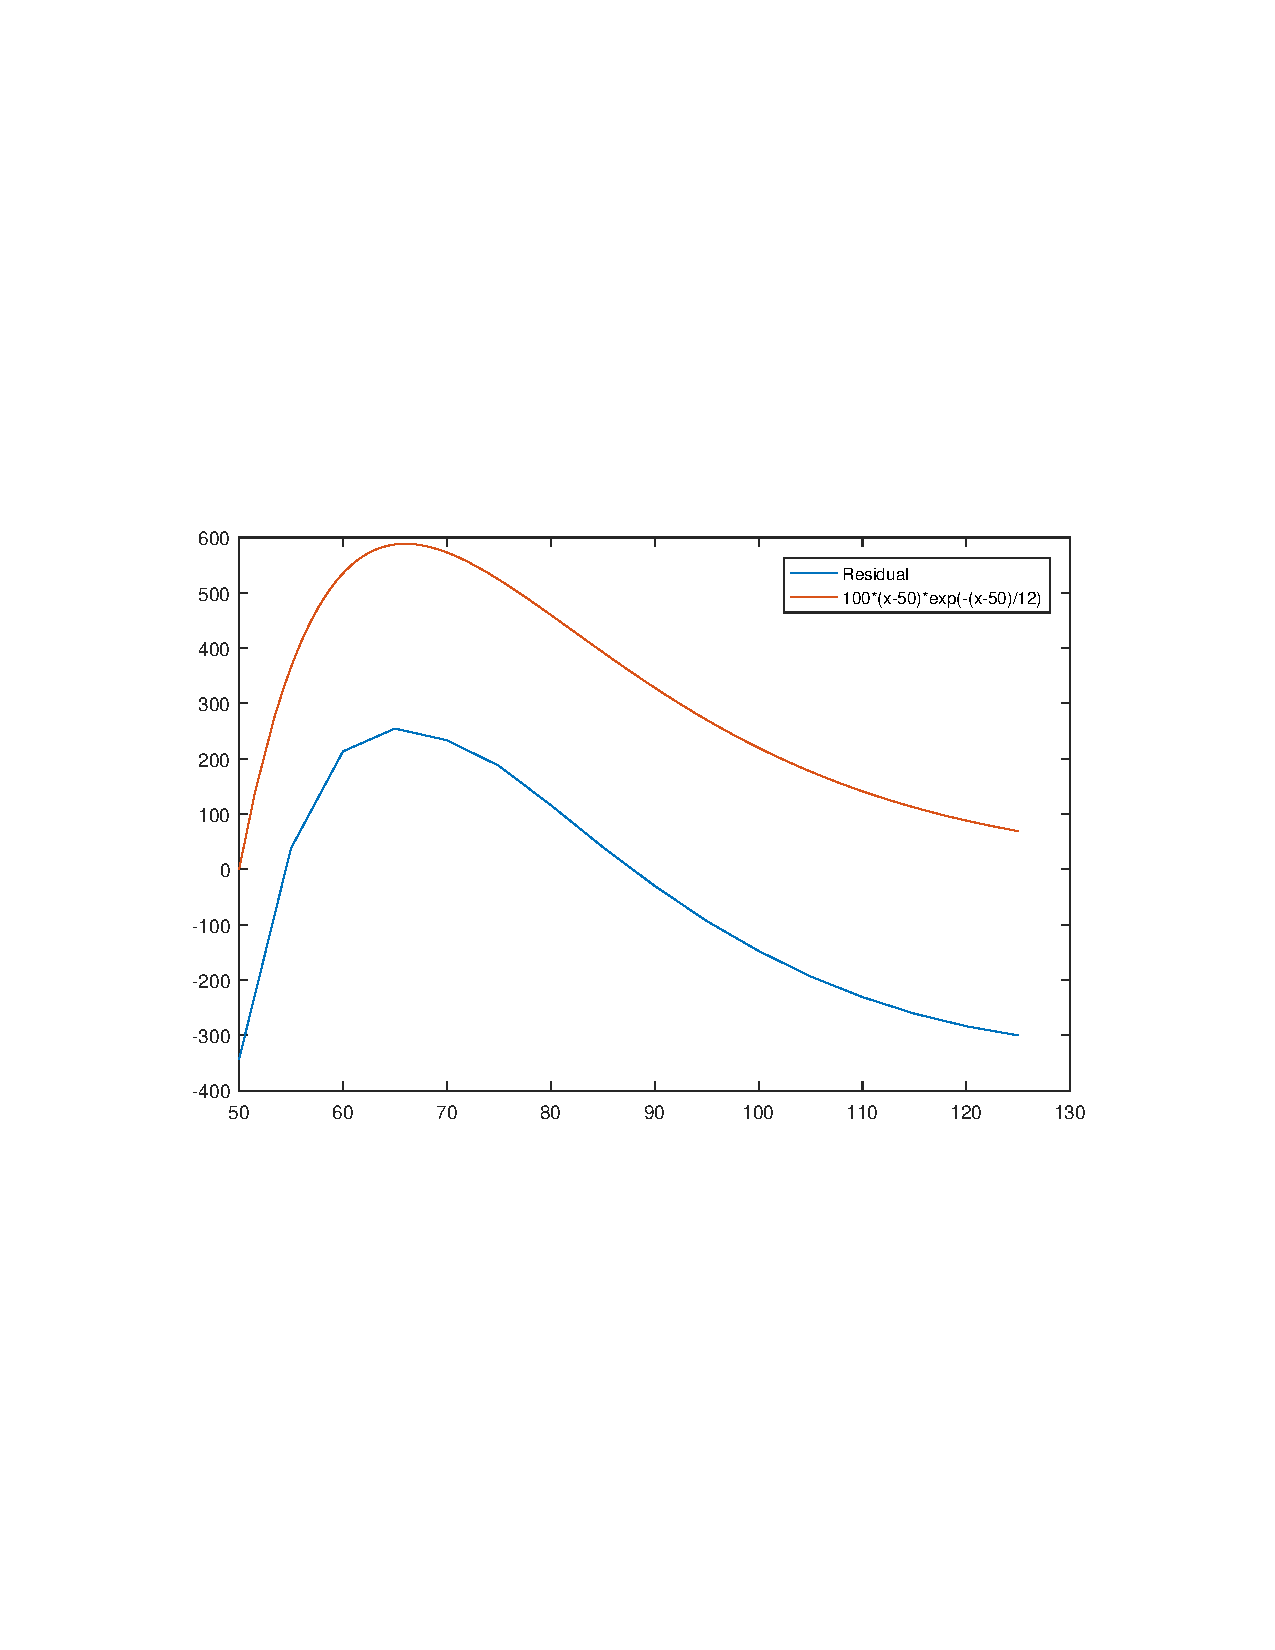
\includegraphics[width=\textwidth]{P2p1.pdf}
	\else
		\includegraphics[width=\textwidth]{P2p	1.eps}
	\fi
	\caption{The residual of the regression with the obtained estimators}
	\label{residual}
	\end{figure}

This has nearly the same shape as
\[	r=100(x-50)\exp\left(-\frac{x-50}{12} \right), \]
which is totally different from the regression model
\[	y=\alpha\exp\left(\frac{\beta}{x+\gamma}\right). \]
Thus, we can accept this residual.	


\section{Conclusions}

When fixed-point iteration does not converge, secant method is more stable to find some good results, although it converges slower than Newton's method.
Furthermore, when all the three numerical methods do not converge, the brute-force method is a reliable alternative, and scanning the log of the output is also a good method, although the are slow and attempt to solve by a computer science approach instead of a numerical method approach.
The results from brute-force method and scanning the log can be good initial guess for Newton's method and secant method.




\newpage
\begin{appendices}
\renewcommand{\thesection}{\Alph{section}}
\section{Appendix}
\subsection{MATLAB\texttrademark\ Function Implemention of the Numerical Methods}

\subsubsection{Fixed-point iteration}
\lstinputlisting[style=Matlab-editor]{mcode/fixedpoint.m}

\subsubsection{Newton's method}
\lstinputlisting[style=Matlab-editor]{mcode/newton_Highdim.m}
\newpage
\subsubsection{Secant method}
\lstinputlisting[style=Matlab-editor]{mcode/secant_Highdim.m}


\subsection{MATLAB\texttrademark\ log of the project}
\lstinputlisting[style=Matlab-editor]{mcode/Project2.m}

\end{appendices}